\chapter{客户参与} % Introduction chapter suppressed from the table of contents

\hypertarget{ux5e38ux89c1ux95eeux9898}{%
\subsection{常见问题}\label{ux5e38ux89c1ux95eeux9898}}

某软件外包开发中心专注承接某政府医疗机构的IT系统维护工作,因为工作量变化很大,而且需要快速反应,一直都是使用敏捷(Scrum)开发方式,每两周一个迭代。但因为甲方提需求的代表都是医护专业,缺乏软件开发和业务分析经验,很多时候,每轮迭代提出的需求都很粗。例如护士办理病人住院:只发出一张表,列举了各种人群患者的入院要求、步骤与条件。 

乙方本来只使用敏捷开发的用户故事(User Story) 方式,
``护士办理病人住院''只算一个用户故事,难以判断:

\begin{itemize}
\tightlist
\item
  需求是否完整。
\item
  与其他功能的依赖关系。(例如如可能有高度传染病,便必须先做某些化验,如果阳性便必须去隔离病房)
\item
  各种异常情景应怎样处理。
\end{itemize}

为了避免开发出来的功能不能满足需求,必须靠乙方开发团队先做好详细分析,但他们反而不太懂业务,导致只能从技术角度分析,未能全面挖掘业务特性。

\hypertarget{ux6539ux8fdbux65b9ux6848}{%
\subsubsection{改进方案}\label{ux6539ux8fdbux65b9ux6848}}

\begin{itemize}
\tightlist
\item
  使用功能点识别实体与行为

  \begin{itemize}
  \tightlist
  \item
    便能容易识别出需求中,哪些地方甲方没有考虑,例如,除了新增,是否也需要有查询和删除功能。
  \end{itemize}
\item
  再利用用例(Use cases)
  与各种场景(Scenarios)和对应系统页面原型图,与甲方代表讨论各种场景,系统应如何处理
\end{itemize}

\hypertarget{ux6539ux8fdbux6548ux679c}{%
\subsubsection{改进效果}\label{ux6539ux8fdbux6548ux679c}}

\begin{itemize}
\tightlist
\item
  挑了两个医疗相关的团队做试点,在开发前预先用了这些方法与甲方充分讨论,3个月6轮迭代后,UAT里的需求相关缺陷数平均降低43\%。
\end{itemize}

从以上案例看到,客户代表除了要参与,还要有具体措施做好需求,例如可利用功能点方法,用例与场景来挖掘分析需求。

\hypertarget{ux8bc6ux522bux5229ux76caux76f8ux5173ux8005}{%
\subsection{识别利益相关者}\label{ux8bc6ux522bux5229ux76caux76f8ux5173ux8005}}

和杭州客户领导吃晚饭,领导就跟同桌的项目经理开玩笑说:``你们刚刚完成内部项目管理自动化工具,做调研的时候好像没有找过我?
其实我是其中一位经常要使用这系统的管理者,下面项目的监控、申请都是经过我,但我发现这个系统很不合用,对收集我需要的项目信息没有作用。比如没办法处理一些批准信息。''\\
从上面对话,可以了解如果没有全面识别项目的利益相关者,可能会影响到项目的成败。例如我接触一些有些具备开发经验的需求人员,但他们通常只注意功能需求的技术细节。

问他们:“哪些是你的项目干系人?”\\
很多人都会说:“甲方有协调员,要访谈哪些人都是由甲方协调员安排,我们听他安排。”所以为了避免未能识别所有干系人的风险,就要主动跟甲方一起策划。我们说沟通计划必须是甲乙方一起合作做出来,而且会牵涉甲乙方各个层次的人。\\
例如要听甲方出资人的需求,可能就要乙方的总经理出马,乙方的需求人员顶多可以跟甲方对口的项目组人员沟通。(如何可以做好识别干系人,并制订沟通计划,可详见附件。)

\hypertarget{ux7528ux6237ux6545ux4e8bux5361}{%
\subsection{用户故事卡}\label{ux7528ux6237ux6545ux4e8bux5361}}

用户故事卡目的是让用户(业务)与开发沟通交流。

虽然Kent
Beck先生强调用户故事卡片上的东西并非交流的全部,也不应该包括太多细节。但XP/Scrum的用户故事卡片未能全面包括需求的各元素,例如缺乏以下内容:

\begin{itemize}
\tightlist
\item
  来源: 每项需求都应可追溯到源头。
\end{itemize}

\begin{itemize}
\tightlist
\item
  冲突:确保需求之间的一致性。
\end{itemize}

\begin{itemize}
\tightlist
\item
  顾客满意度 /
  顾客不满意度:用两个数比单纯用优先级能更全面反应客户声音。
\end{itemize}

%\href{文件:9_用户故事1.png}{450px}

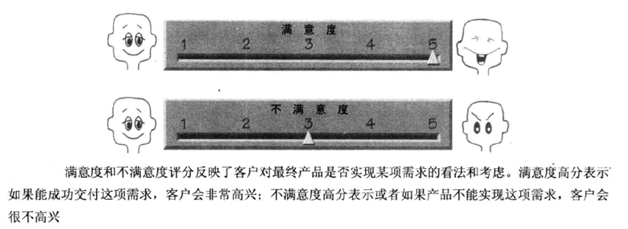
\includegraphics[width=6cm]{9_用户故事1.png}

\begin{description}
\tightlist
\item[]
(如想多了解为什么要这样分,请看附件里的``客户声音: Kano Diagram'')
\end{description}

卡片例子可参考ROBERTSON夫妇的需求卡片模板:

%\href{文件:9_用户故事2.png}{500px}

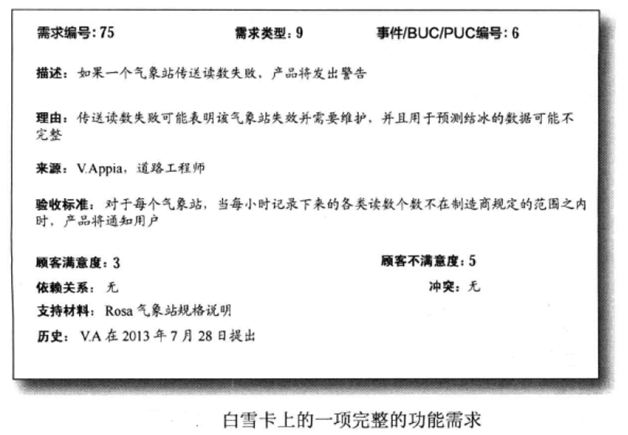
\includegraphics[width=6cm]{9_用户故事2.png}

也可以用于非功能需求:\\
%\href{文件:9_用户故事3.png}{500px}

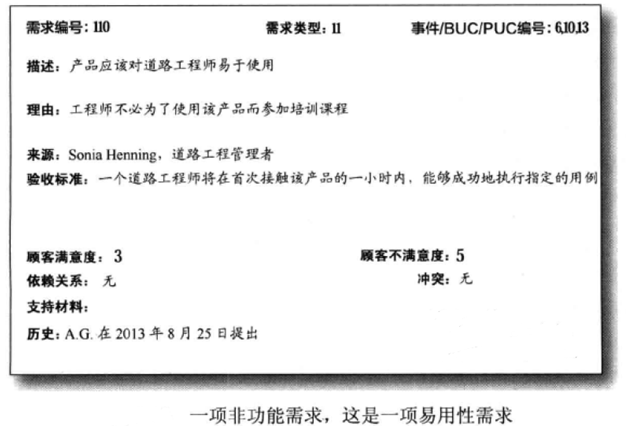
\includegraphics[width=6cm]{9_用户故事3.png}

\begin{itemize}
\tightlist
\item
  千万不要误以为卡上的所有信息都需要一次性与用户获取。
\item
  挖掘需求永远是持续,并不断细化。
\item
  卡片上增加了这些部分,可提醒我们不要忽略这些元素。
\end{itemize}

\hypertarget{ux7528ux4f8bux4e0eux573aux666f}{%
\subsection{用例与场景}\label{ux7528ux4f8bux4e0eux573aux666f}}

用户故事针对 ``做什么''与 ``为什么'' ("What", "Why");
用例与各种场景针对``如何做'' ("How" ),所以它们之间是互补,没有冲突。

下面用大家都熟悉的简单系统``在核酸检查点做检查并提交结果''来举例说明,如果考虑不周全,也会导致需求相关问题。

%\url{文件:CI场景图.jpg}

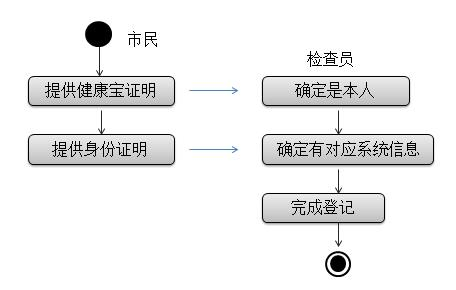
\includegraphics[width=6cm]{CI场景图}

\textbf{正常情况}:使用身份证时,用读卡器获取实名身份信息,与系统记录对应,记录信息也齐全,包括手机号码。\\
\textbf{其他可选情况}:没有身份证,可用其他证件,例如港澳通行证、国外护照。\\
\textbf{异常情况}:市民身份信息不能用读卡器自动获取,需要手工输入,但检察员输入信息错误。例如护照号码错误,手机号码为空,被删掉或者没输入。\\
如果问需求分析师、产品经理有什么异常场景,一般都会回应``没有'';部分回应一些最基本的异常,例如``只有输入信息错误、报错,要求重新输入'',我便会以我的经验举例,说明必须要识别各种异常场景,才能算全面挖掘需求;识别正常场景是基本工,能识别各种异常场景才算做好。

\framebox{%
\begin{minipage}[t]{0.97\columnwidth}\raggedright
我每次在北京做免费核酸检测,因为非身份证,检测员都要用手机手工输入我的信息:
姓名和港澳通行证号(因为系统已经有我的手机号,所以通常不需要再输入手机号),
只要我确认以上信息都输入正确,通常都没有问题。

后面不知道什么原因?
不再用手机,改用笔记本电脑配电子读卡器阅读电子身份证和电子扫描器读二维码。

检测员不再要手工输入我的信息, 靠我预先进系统填好所有信息,生成二维码,
只要检测员验证了我的二维码信息与系统信息对应,便可完成。

一般正常操作是没有问题的。

但我最近在某采集点检查完,之后第二天未能在我健康宝正确展示出核酸结果。(开头以为出现了``混管阳性'',但之后几次核酸结果又回复正常。)

我遇到的问题可能是因为那个采集点使用了笔记本电脑,信息先存在电脑,最后才批量上传到服务器。但因为非身份证的情况,没有检查清楚信息是否都完备,例如,可能某些信息被检察员错误删掉了,但电脑没有报异常,最终批量上传时,服务器便无法识别我的检查记录。
以上只是我的猜测,估计永远都不会知道真正答案,但无论如何,如果当初系统分析时能全面识别所有场景,应可避免这类问题。
\strut
\end{minipage}}

\framebox{%
\begin{minipage}[t]{0.97\columnwidth}\raggedright
如果使用银行交易系统概念,应可避免这类错误。比如我从自己账号转钱到另一个人的账号,中间会经过多家银行,我提交后,系统都会确保中间每一轮交易都已成功完成,并确认对方银行最终收到款,才算完成这个交易(通常前后经过几分钟)。中间任何环节出问题,都会撤回整个交易,能避免出现我那种不了了之的情况了。

\strut
\end{minipage}}

如果信息有误或者不成功,导致最终无法提交上线,怎么处理?因总服务器本身或网络出问题无法连上,怎么处理?\\

如果要充分考虑各种异常情况,应仔细询问以下一系列问题:\\


\framebox{%
\begin{minipage}[t]{0.97\columnwidth}\raggedright
通过检查正常情况的每一步井询问以下问题,可以发现异常情况。

\begin{itemize}
\tightlist
\item
  如果这一步不能完成,或没有充成,或得到了错误,不可接受的结果,会发生什么?
\item
  在这一步会发生什么错误?
\item
  会发生什么事情,阻止工作到达这一步?
\item
  是否有一些外部实体可以打断或阻止这一步,甚至这个业务用例?
\item
  实现这一步的技术是否会失败或不可使用?
\item
  最终用户是否会不理解对他们的要求,或者错误地理解产品提供的信息?
\item
  最终用户是否会采取错误的行动(有意或无意),或者没有做出响应?
\end{itemize}
\strut
\end{minipage}}

另外一类情况,有几十人排队等待做核酸,原因是服务器出了问题,停机了,排队人非常不满。工作人员也很尴尬说已经想尽办法用手机、电脑,但是都没办法。如果提前想好这种场景,就可以在本地把相关信息记录下来,等服务器恢复后一次性上传,就可以避免刚才的情况。\\
除了正常,也可以考虑一些\textbf{假设的场景},让干系人、客户可以更开放地考虑各种不同的情况,更创新。例如是否可以考虑像超市付款一样,自主处理?当很多人排队的时候,就不会因为检察员一个人忙不过来,导致排长队。\\
例如取登机牌也可以用机器,让乘客自主一组办理。其实做核酸也可以这样处理。\\
所以从以上案例看到用例+场景不同于用户故事,可以弥补后者。Kent
Beck先生特别提倡用户故事,因为当时很多客户都觉得用例太细、太偏技术,不愿意写,甚至也不愿意读;但客户大多都愿意用自然语言写用户故事,可以很容易触发客户与开发交流沟通。

但如果需求分析师只考虑现在业务流程的各种场景,开发人员开发系统,把所有的场景都覆盖好,是否便能成功?
不一定,请看以下例子:

\hypertarget{ux4e3eux4f8b}{%
\subsection{举例}\label{ux4e3eux4f8b}}

你们都有申请过护照吗?
比如我们护照更新,以前是要到柜台手工办理,如果我们把那个过程数字化,应该怎么做呢?

某国家的做法是本来的手工填写模板直接变成系统页面(每个输入与手工表格一一对应),申请人在系统里按本来模板填写并提交,上传个人新照片,也是经过系统,我有一次尝试用系统线上填电子表单申请,但因表单很繁琐,有很多护照原有信息都需要重新填写,光是填那表就花了我接近一个小时,最大问题还不是在我花时间填手工表,而是最后要上传照片,因为照片像素高的话就很大,需要很好的网络才可以传得上,如果照片像素小,便导致模糊不清,不能通过。最后,一个半小时后,我用尽所有方式都还是无法传上照片,我最终放弃了在线上提交申请,直接预约去在柜台做!\\
客户:有好方法解决这问题吗?\\
我:有,另外某国家的做法就很简单多了:\\
之前描述的整个过程只是把原有的手工步骤信息化,和原本的申请手续一样。但线上办理和在柜台现场办理不同,在现场你可以要求对方直接把照片给你,也可以要求对方提供老护照,但在线上办理,应很容易从系统里找到个人护照信息,所以很多本来在柜台要手工填写的老护照信息就不需要再填了。\\
客户:怎么可以简化整个过程?最困难应是照片的更新?\\
我:有些国家是这样做法,比如你申请续证,只需要填上老证件的基本信息,系统就立马能识别出本来的证件
你确实有那个``旧''证后,便可立马提交申请。跟在网上购物一样,你确认过内容没问题,就在网上付费,然后打印申请表并在表上亲手签字,然后附上几张符合规格的照片,邮寄到政府机关。他做好新证件以后再邮寄回你。或者你自己到他规定的地点领取也可以。这样就能很简单地利用``低''科技解决方案,解决了刚才上传照片的困难。

从上面例子看到,我们应不仅是把那些本来手工的流程自动化,应该全局看要解决的问题本身,哪些过程自动化,哪些不应该自动化(比如传照片)。

甲方对怎么可以在线上做这个过程也没有概念,他只是知道,本来手工需要填表。
乙方也不知道,他只是做开发,也不知道有什么方面可以不用IT方式,而用其他方式更合理。
必须要一起探讨才可以有最好的解决方法。

所以作为业务分析师,你很可能要改变用户思考问题的方式,例如利用业务过程模型,配合场景与页面原型,与利益相关者一起探索问题的本质。软件系统必须为拥有它的人提供最理想的价值,构建软件系统本身(例如只是把现有流程自动化)不一定能解决客户业务问题。

\hypertarget{ux5e38ux89c1ux95eeux9898}{%
\subsection{结束语}\label{ux5e38ux89c1ux95eeux9898}}

除了有客户参与团队,快速反馈,也要:

\begin{itemize}
\tightlist
\item
  全面识别所有利益相关者。
\item
  利用功能点分析,了解范围,确保需求完整。
\item
  利用用例与各类场景,全面了解各业务事件都可度量、可测试。
\item
  利用需求卡片记录用户故事
  (因与干系人沟通,获取需求是持续逐步细化过程)。
\end{itemize}

\hypertarget{ux9644ux4ef6}{%
\section{附件}\label{ux9644ux4ef6}}

\hypertarget{ux5229ux76caux76f8ux5173ux8005}{%
\subsection{利益相关者}\label{ux5229ux76caux76f8ux5173ux8005}}

\hypertarget{ux5229ux76caux76f8ux5173ux8005ux8ba1ux5212ux68c0ux67e5ux5355-stakeholders-plan-checklist}{%
\subsubsection{利益相关者计划检查单 (Stakeholders Plan
Checklist):}\label{ux5229ux76caux76f8ux5173ux8005ux8ba1ux5212ux68c0ux67e5ux5355-stakeholders-plan-checklist}}

1)列出所有潜在的利益相关者 (List all potential stakeholders)\\
1a. 类型 / 分组 (What are the base Segments)\\
1b. 可否再细分 (Any sub-segments)\\	
2)把她们分为 F(友好),I(忽略),U(不友好)\\
Assign F (Friendly), I (Ignore), U (Unfriendly) to them\\
3)他们最关注什么?

\begin{description}
\tightlist
\item[]
What is important to them?\\
\end{description}

4)学习目标 (Learning objectives):\\
针对某利益相关者,我们需要了解什么\\
For each stakeholder, what will we need to learn?\\	
5)怎样沟通 (How)\\
6)什么时间 (When)\\
7)抽样计划 (Sampling plan)

\begin{description}
\tightlist
\item[]
如何招募 (How to recruit)\\

如何能获得承诺 (How to get commitment)\\
\end{description}

\begin{description}
\item[]
\begin{description}
\tightlist
\item[]
{[}针对以上第一至第三项,参阅以下实例/解读{]}
\end{description}
\end{description}

\hypertarget{ux5b9eux4f8bux89e3ux8bfb-examples-explanation}{%
\subsubsection{\texorpdfstring{\textbf{实例/解读 (Examples /
explanation)}}{实例/解读 (Examples / explanation)}}\label{ux5b9eux4f8bux89e3ux8bfb-examples-explanation}}

某公司专门设计、开发新一代手提电脑产品。

1/ 全面考虑各类利益相关者Stakeholders\\
%\href{文件:7_利益相关者1.png}{文件:7 利益相关者1.png}
%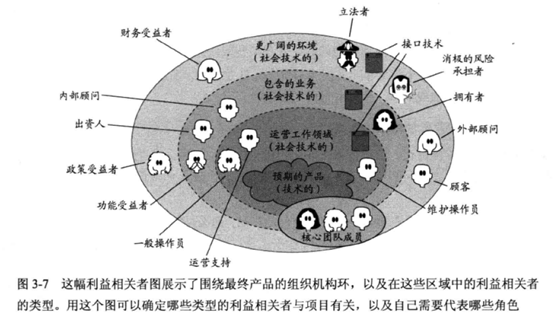
\includegraphics[width=6cm]{7_利益相关者1.png}
\textbf{出资人 (Sponsor):}出资人为产品的开发付钱\\
\textbf{顾客
(Customer):}顾客购买产品。必须对他们有足够的了解,理解他们认为什么有价值,所以会购买什么产品。\\
\textbf{用户
(User):}确定用户的目的是为了理解他们所做的工作,以及他们认为哪些改进有价值。\\
在开发消费产品、大市场软件时,应该考虑用一个\textbf{``假想用户''}。假想用户是一个虚拟用户,他是大多数用户的原型。\\
类型/分组的例子:\\
\textbf{未来笔记本电脑的潜在用户}:\\
大类:\\

\begin{enumerate}
\tightlist
\item
  商业人士 (Business)
\item
  媒体专业人士(Media Pro)
\item
  家庭用户(Home)
\end{enumerate}

细分:\\

\begin{enumerate}
\tightlist
\item
  主要用户(Lead User)
\item
  有极高要求者(有挑战的 Demanding)
\item
  潜在用户(有潜力的 Potential)
\item
  追求技术完美者 (技术流 Tech-Phobic)
\end{enumerate}

%\href{文件:CustomerMatrixScreenshot_2022-12-16_180326.jpg}{500px}

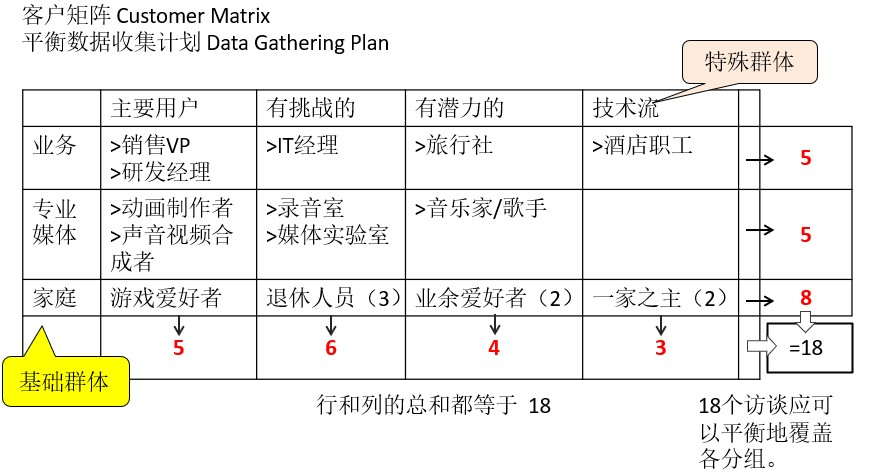
\includegraphics[width=6cm]{CustomerMatrixScreenshot_2022-12-16_180326.jpg}
 	
2) 策划包括哪些用户(User inclusion strategy)\\
依据设计人员会怎么对应,把不同识别出来的利益相关者分成
\textbf{F}、\textbf{I}、\textbf{U}\\
例:以针对笔记本电脑创新产品\\
\textbf{F(Friendly)友好},比如家庭用户、商业用户、媒体专员\\
\textbf{I(Ignore)忽略} ,比如忽略残疾人士\\
\textbf{U(Unfriendly)不友好},比如黑客、小孩(禁止他下载游戏、玩游戏)\\	
3)  他们注重什么(主要关注点)

%Screenshotfrom2023-11-0302-49-29.png

%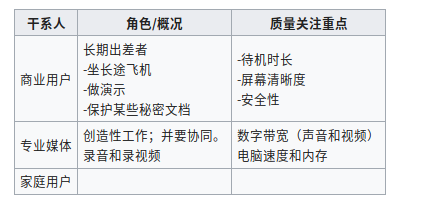
\includegraphics[width=6cm]{Screenshotfrom2023-11-0302-49-29.png}

\begin{tabular}{|c|c|c|}
\hline
干系人&角色/概况&质量关注重点\\
\hline
商业用户&长期出差者
-坐长途飞机
-做演示
-保护某些秘密文档&-待机时长
-屏幕清晰度
-安全性 \\
\hline
专业媒体&创造性工作;并要协同。
录音和录视频&数字带宽(声音和视频)
电脑速度和内存  \\
\hline
家庭用户&\:&\:\\
\hline
\end{tabular}

\begin{itemize}
\tightlist
\item
  以上有那些在调研之前已知,其他有那些需要挖掘。
\end{itemize}

\hypertarget{ux5ba2ux6237ux58f0ux97f3kano-diagram}{%
\subsection{客户声音:Kano
Diagram}\label{ux5ba2ux6237ux58f0ux97f3kano-diagram}}

可以用下图分析用户对需求优先级:

%\href{文件:IcKanoDiagramScreenshot_2022-12-17_120845.2.jpg}{600px}

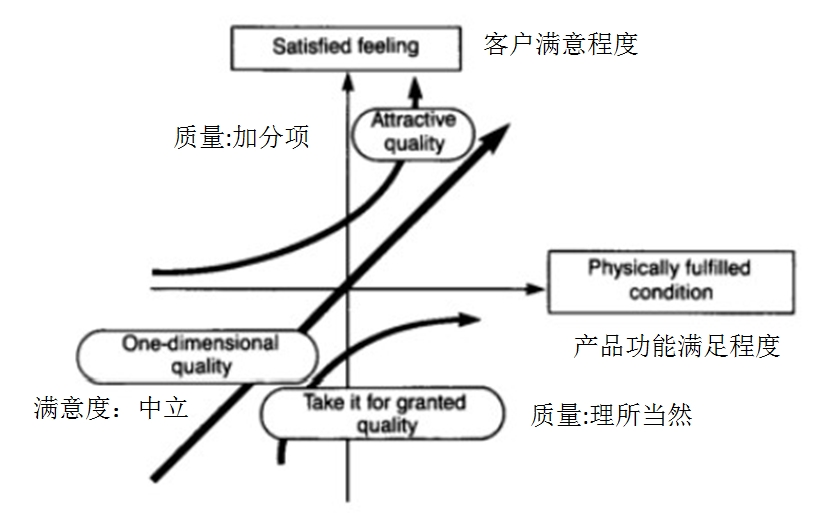
\includegraphics[width=6cm]{IcKanoDiagramScreenshot_2022-12-17_1208452.jpg}

解读上下两个箭头应怎样看:\\
*下面的箭头代表理所当然(Take it for
granted),如果缺乏,客户会很不满意,包括觉得是理所当然
(例如满意度:中立1,非常不满5) 。

\begin{itemize}
\tightlist
\item
  上面的箭头代表是加分项
  (Attractive),如果包括会非常满意,但如果缺乏不会觉得不满意
  。(例如满意度:非常满意5 ,不满意度:中立1)。
\end{itemize}

所以``需求卡片''用两个系数:顾客满意度+顾客不满意度,能更好判断某功能属于哪类功能需求。

\hypertarget{ux9644ux4ef6}{%
\section{参考 References}\label{ux9644ux4ef6}}

1. Beck, Kent , with D. West. "User Stories in Agile Software Development" , Ch.13 of  ''Scenarios, Stories, Use Cases: Through the Systerms Development Life-Cycle''edited by F. Alexander(2004)\\
2. Cohn, Mike . ''User Stories Applied.  ''(2004)\\
3. Martin, Robert C. ''Clean Agile - Back to Basics.''\\
4. Robertson, S.  ''Mastering the requirements process. '' (2006) 2/e\\



